\chapter{Anwendung statistischer Methoden}

In diesem Kapitel werden nun mehrere Programmiersprachen vorgestellt, die sich für Regressionsanalyse eignen. Im letzten Teilkapitel wird demonstriert, wie man solche Methoden mit vorhandener SQL-Syntax umsetzen und durchführen kann.

\section{Beispieldaten}

Um Regressionsanalyse auch praktisch betreiben zu können, arbeiten wir in dieser Arbeit mit einem Satz an Beispieldaten. Diese Daten wurden mit einem Python-Skript erstellt, welches im als Ganzes im Anhang zu finden ist. Dabei werden die einzelnen Merkmale eines Datensatzes mit Absicht so erstellt, dass eine Korrelation zwischen diesen bewusst erzeugt oder nicht erzeugt wird. Diese Beispieldaten liegen in Form einer csv-Datei vor, welche in jeder Sprache einfach eingelesen werden kann.

Wir betrachten hier fiktive Kunden von Amazon. Für jeden Kunden wissen wir das Alter, die Anzahl seiner Käufe, die Summe des ausgegebenen Geldes und ob der Kunde Amazon-Prime Mitglied ist oder nicht. Der ausgegebene Betrag wird in Cent angegeben, um mit ganzen Zahlen rechnen zu können. Die Prime-Mitgliedschaft wird mit einer 1 symbolisiert, während eine 0 das Gegenteil bedeutet.

Insgesamt wurden für diese Arbeit 100.000 solcher Datensätze erzeugt. In der folgenden Tabelle sind die ersten 10 Datensätze beispielhaft dargestellt.

\begin{center}
  \begin{tabular}{|c|c|c|c|}\hline
    \textbf{age} & \textbf{purchases} & \textbf{money} & \textbf{prime} \\ \hline
    30 & 1 & 4421 & 0 \\ \hline
    30 & 11 & 23346 & 1 \\ \hline
    33 & 1 & 4010 & 0 \\ \hline
    31 & 19 & 52517 & 1 \\ \hline
    29 & 3 & 8046 & 0 \\ \hline
    28 & 12 & 25295 & 0 \\ \hline
    41 & 16 & 38236 & 1 \\ \hline
    23 & 3 & 7098 & 1 \\ \hline
    25 & 1 & 2707 & 0 \\ \hline
    38 & 20 & 50976 & 1 \\ \hline
  \end{tabular}
\end{center}

Wir definieren uns außerdem drei Fragestellungen, welche wir jeweils mit einer Art der in Kapitel 2 vorgestellten Regressionen beantworten werden:
\begin{enumerate}
  \item Zuerst wollen wir wissen, ob das ausgegebene Geld mit der Anzahl der Käufe in Zusammenhang steht. Diese Fragen können wir mit einfacher linearer Regression beantworten. $money$ ist hierbei die abhängige Variable und $purchases$ ist die unabhängige Variable.
  \item Die zweite Frage ist ähnlich der ersten, nur wollen wir hier wissen, ob neben der Anzahl der Käufe auch das Alter des Kunden einen Einfluss auf das ausgegebene Geld hat. Hier haben wir nun zwei unabhängige Variablen, nämhlich $age$ und $purchases$. Die abhängige Variable bleibt $money$. Diese Frage beantworten wir also mit multipler linearer Regression.
  \item Als letztes interessiert uns, ob eine Prime-Mitgliedschaft von der Summe des ausgegebenen Geldes zusammenhängt. $money$ ist also nun die unabhängige Variable, während $prime$ die abhängige Variable ist. Außerdem ist $prime$ eine binäre Variable. Deshalb nutzen wir hier also logistische Regression.
\end{enumerate}


\section{Regression in R}
Das R-Projekt oder einfach nur R ist eine Sprache für statistische Berechnungen und graphische Darstellung. Damit ist R wie geschaffen für Regressionsanalyse. Von allen hier behandelten Sprachen ist R damit auch die einfachste und direkteste für Regression.

In R sind einfache Datenstrukturen wie Vektoren, Matrizen und Listen als Datentypen vorhanden. Darauf aufbauend existieren sogenannten Dataframes. Diese sind eine Liste von Vektoren der gleichen Länge und werden gerne zur Repräsentation von Datentabellen verwendet. Die Vektoren der Liste entsprechen dann den Spalten der Tabelle.

In R lassen sich außerdem sehr einfach sogenannte Modelle definieren, welche als Eingabe nur die Daten und eine Formel benötigen. Eine Formel ist von der Form $y \sim modell$ und enthält den funktionalen Zusammenhang zwischen der abhängigen und den unabhängigen Variablen.

\subsection{Einfache lineare Regression}

Betrachten wir also Frage Nummer $1$ aus dem vorherigen Teilkapitel. Die Formel lautet dann einfach $money \sim purchases$. Um die Parameter zu berechnen sind nur wenige Zeilen R-Code nötig. Man liest die Daten aus der csv-Datei, erstellt das Modell mit der Formel und berechnet die Parameter. Die print-Funktion druckt am Ende das Ergebnis:

\begin{lstlisting}
  data <- read.csv2("sample.csv", sep = ",", header = TRUE)
  modell <- as.formula("money ~ purchases")
  slr <- lm(modell, data = data)
  print(slr)
\end{lstlisting}

R verfügt auch über Möglichkeiten zur graphischen Darstellung. Lässt man die die Datenpunkte und die lineare Ausgleichsfunktion mit den berechneten Parameter plotten, erhält man dieses Ergebnis:

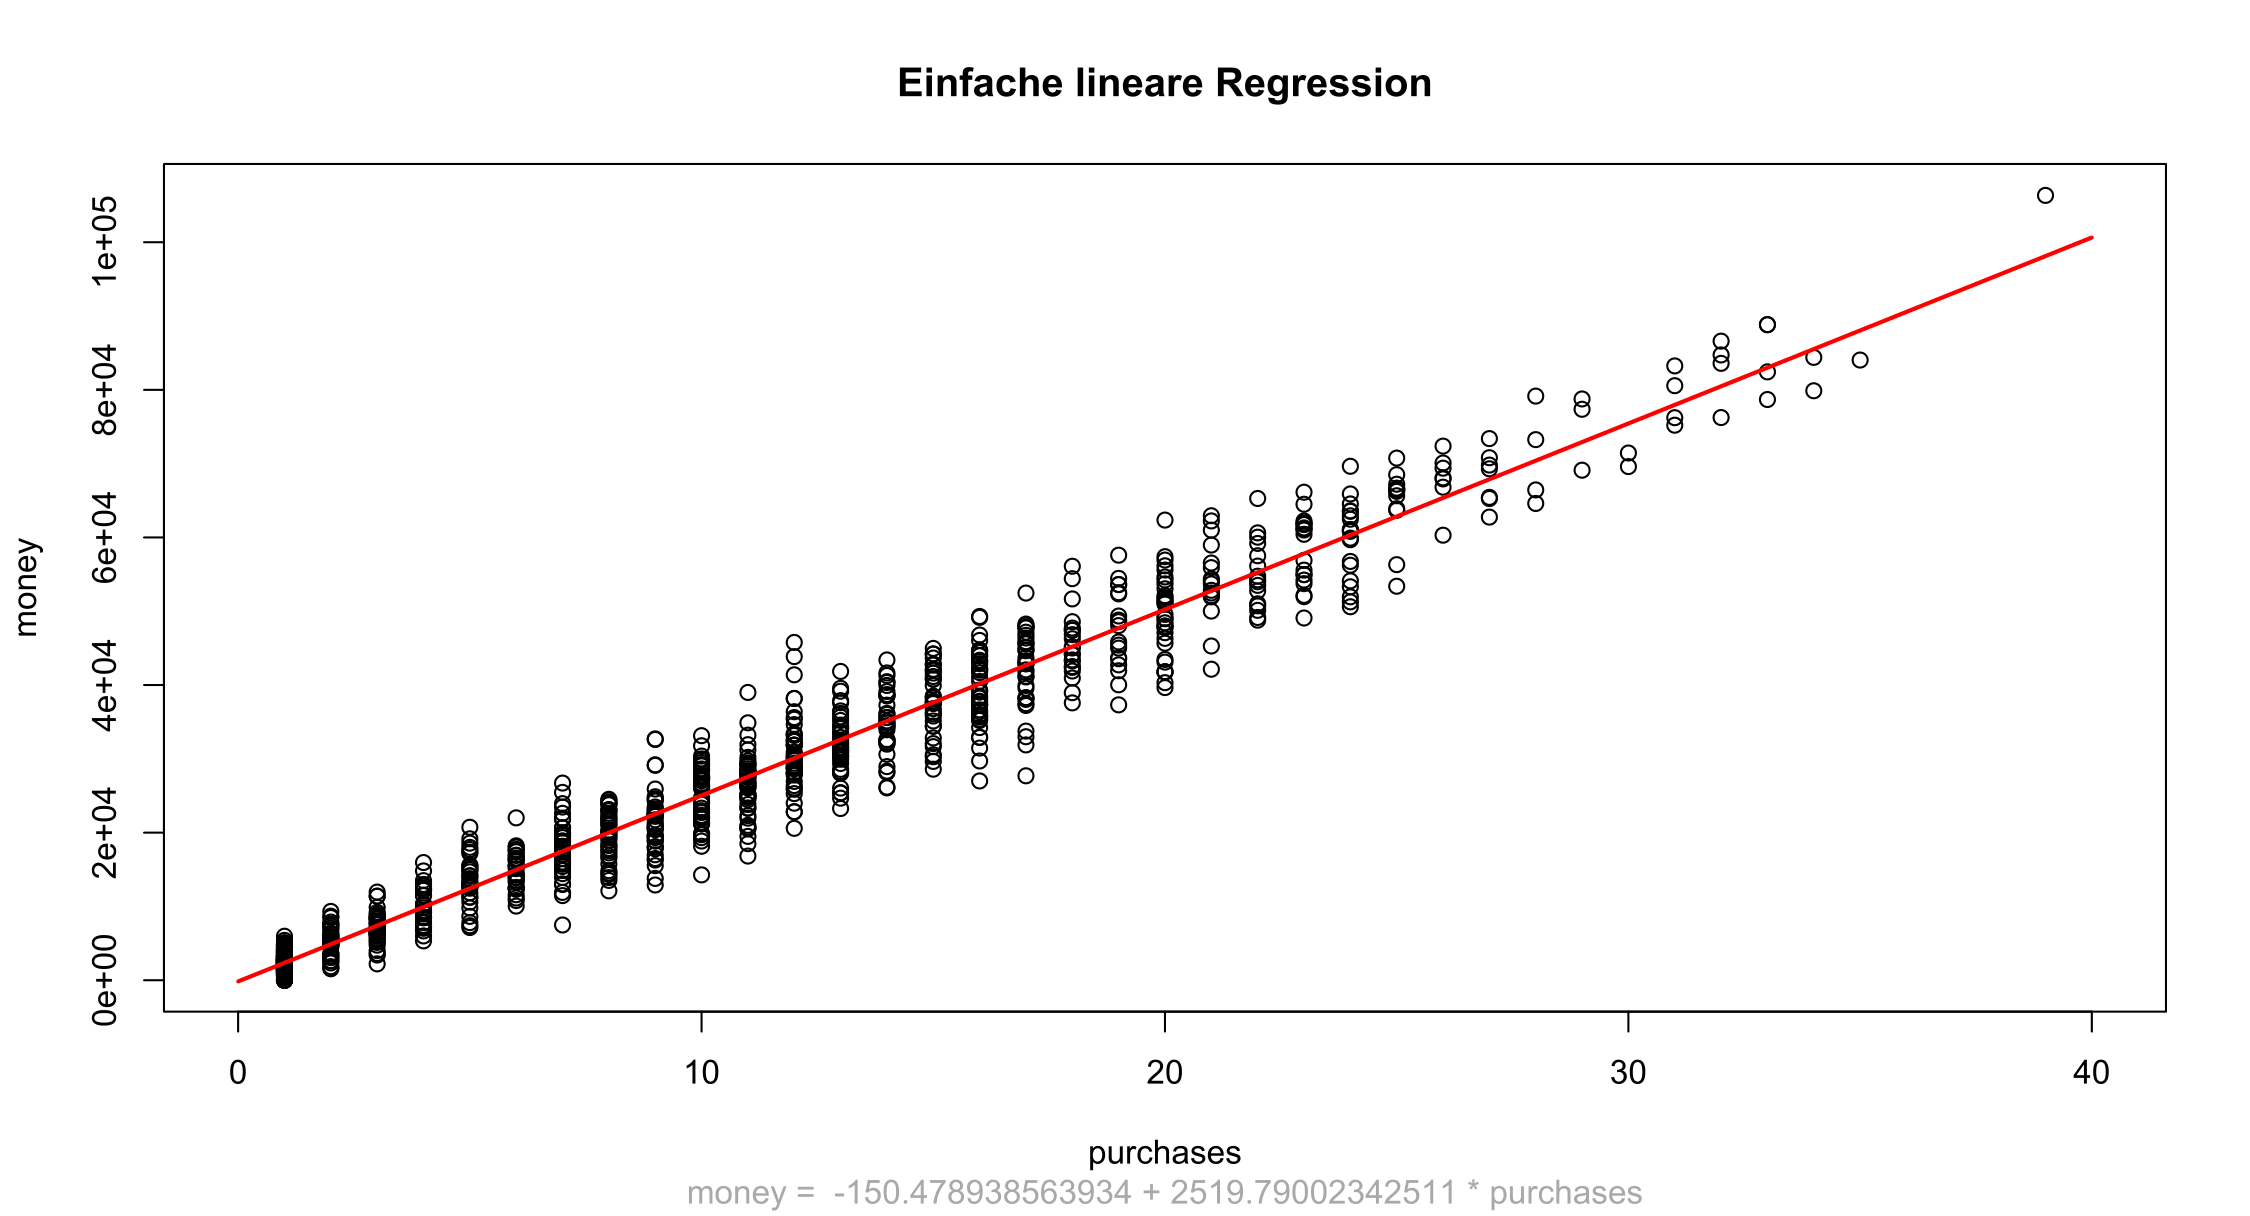
\includegraphics[width=\textwidth]{r-simpleLinearRegression}

\subsection{Multiple lineare Regression}

\subsection{Logistische Regression}

\section{Regression in Tensorflow}

\subsection{Einfache lineare Regression}

\subsection{Multiple lineare Regression}

\subsection{Logistische Regression}

\section{Regression in SQL}

\subsection{Einfache lineare Regression}

\subsection{Multiple lineare Regression}

\subsection{Logistische Regression}
